\section{Experimental results}
\label{sec:experiments}

\subsection{Arithmetic datasets}

The arithmetic dataset is a replica of the "simple function task" as shown in \cite{trask-nalu}.
The goal is to sum two subsets of a vector and perform a arithmetic operation as defined below
\begin{equation}
t = \sum_{i = a_{\mathrm{start}}}^{a_{\mathrm{end}}} \mathbf{x}_i \circ \sum_{i = b_{\mathrm{start}}}^{b_{\mathrm{end}}} \mathbf{x}_i \quad \text{where } \mathbf{x} \in \mathbb{R}^n, x_i \sim \mathrm{Uniform}[r_{\mathrm{lower}}, r_{\mathrm{upper}}], \circ \in \{+, -, \times\}
\label{eq:arithmetic-problem}
\end{equation}
where $n$, $r_{\mathrm{lower}}$, $r_{\mathrm{upper}}$, $\circ$, the subset size, and subset overlap are dataset parameters that we use to test the models ability to learn.
We define a set of default parameters (see table \ref{tab:simple-function-task-defaults}).
When probing a specific dataset parameter, e.g. subset overlap, the default will be the used for the remaining parameters.
\begin{table}[h]
\caption{Default dataset parameters}
\label{tab:simple-function-task-defaults}
\centering
\begin{tabular}{r l}
\toprule
 Parameter name & Default value \\
 \midrule
 Input size & 100 \\
 Subset ratio & 0.25 \\
 Overlap ratio & 0.5 \\
 Interpolation range & $U[1,2]$ \\
 Extrapolation range & $U[2,6]$ \\
 \bottomrule
\end{tabular}
\end{table}

\subsubsection{Model evaluation}

The goal is to achieve a solution that is acceptably close to a perfect solution. To evaluate if a model instance solves the task, the MSE is compared to a known nearly-perfect solution on the extrapolation range. If $\mathbf{W}_1, \mathbf{W}_2$ defines the weights of the fitted model, and $\mathbf{W}_1^\epsilon$ is nearly-perfect and $\mathbf{W}_2^*$ is perfect (example in equation \ref{eq:nearly-perfect-solution-example}), the success criteria is $\mathcal{L}_{\mathbf{W}_1, \mathbf{W}_2} < \mathcal{L}_{\mathbf{W}_1^\epsilon, \mathbf{W}_2^*}$, measured on the extrapolation error, for $\epsilon = 0.0001$.
\begin{equation}
    \mathbf{W}_1^\epsilon = \begin{bmatrix}
    1 - \epsilon & 1 - \epsilon & 0 + \epsilon & 0 + \epsilon \\
    1 - \epsilon & 1 - \epsilon & 1 - \epsilon & 1 - \epsilon
    \end{bmatrix}, \mathbf{W}_2^* = \begin{bmatrix}
    1 & 1
    \end{bmatrix}
    \label{eq:nearly-perfect-solution-example}
\end{equation}

All experiments are evaluated multiple times with different seeds. We define the success rate as the percentage of experiments that achieves success.

A sparsity error is also evaluated, which is defined in equation \ref{eq:sparsity-error}. This is only considered for model instances that did solve the task, for which the mean and 95\% confidence interval is reported.
\begin{equation}
E_\mathrm{sparsity} = \max_{h_{\ell-1}, h_{\ell}} \min(|W_{h_{\ell-1},h_\ell}|, |1 - |W_{h_{\ell-1},h_\ell}||)
\label{eq:sparsity-error}
\end{equation}

The first iteration for which $\mathcal{L}_{\mathbf{W}_1, \mathbf{W}_2} < \mathcal{L}_{\mathbf{W}_1^\epsilon, \mathbf{W}_2^*}$, is also reported with the 95\% confidence interval. Again, only model instances that did solve the task are considered. 

\subsubsection{Experiment setup}

The multiplication models, NMU and $\mathrm{NAC}_{\bullet}$ have an addition layer first, either NAU or $\mathrm{NAC}_{+}$, followed by a multiplication layer. The addition models, $\mathrm{NAC}_{+}$, NAU, and Linear are just two layers of that unit. Finally, the NALU model is also two layers of NALU. See explicit definitions in table \ref{tab:model-defintions}. All models are fitted with an MSE loss function.

For all experiments $\lambda_{\mathrm{oob}} = 1$ and $\lambda_{\mathrm{bias}} = 0.1 \cdot (1 - \exp(-10^5 \cdot t))$. Gradually scaling the bias regularizer $\mathcal{R}_{\ell,\mathrm{bias}}$ is to ensure it does not interfere with early training. We show the effect of regularization in appendix \ref{sec:appendix:simple-function-task:regualization}. All experiments uses Adam optimization \cite{adam-optimization} with default parameters, and are computed on an HPC cluster using \text{8-Core Intel Xeon E5-2665 2.4GHz} CPUs.

The training dataset is continuously sampled from the interpolation range, a different seed is used for each experiment. Training is done with a mini-batch size of 128 observations. A fixed validation dataset with $10000$ observations is sampled from the interpolation range. A fixed test dataset with $10000$ observations is sample from the extrapolation range.

Validation error, test error and sparsity error is sampled every $1000$ iterations. To avoid noise from exploration, the best fit in terms of the validation error among the last $100$ samples is used.

\subsubsection{Learning a 10 parameter function}

To empirically validate the theoretical challenges with $\mathrm{NAC}_{\bullet}$ consider the very simple problem shown earlier in figure \ref{fig:nac-mul-eps-issue}. That is, $t = (x_1 + x_2) \circ (x_1 + x_2 + x_3 + x_4)$ for $x \in \mathbb{R}^4$.
Effectively having to learn 10 parameters to emulate discrete behaviours for exact addition and multiplication.

For the $\mathrm{NAC}_{\bullet}$, NALU and NMU we conduct 100 experiments with different seeds, and stopped after $2 \cdot 10^5$ iterations.

The results, in table \ref{tab:very-simple-function-results}, show that NMU has a higher success rate and converges faster. When inspecting the $6\%$ that did not converge, we found the issue to be underflow when $w = 0$ in the NMU layer.
\begin{table}[!h]

\caption{\label{tab:very-simple-function-results}Shows the success-rate, at what global step the model converged at, and the sparsity error for all weight matrices, with 95\% confidence interval. Best result is highlighed.}
\centering
\begin{tabular}{crllll}
\toprule
\multicolumn{1}{c}{Op} & \multicolumn{1}{c}{Model} & \multicolumn{1}{c}{Success} & \multicolumn{2}{c}{Solved at} & \multicolumn{1}{c}{Sparsity error} \\
\cmidrule(l{3pt}r{3pt}){1-1} \cmidrule(l{3pt}r{3pt}){2-2} \cmidrule(l{3pt}r{3pt}){3-3} \cmidrule(l{3pt}r{3pt}){4-5} \cmidrule(l{3pt}r{3pt}){6-6}
 &  & Rate & Median & Mean & Mean\\
\midrule
 & $\mathrm{NAC}_{\bullet}$ & $13\% {~}^{+8\%}_{-5\%}$ & $5.5 \cdot 10^{4}$ & $5.9 \cdot 10^{4} {~}^{+7.8 \cdot 10^{3}}_{-6.6 \cdot 10^{3}}$ & $7.5 \cdot 10^{-6} {~}^{+2.0 \cdot 10^{-6}}_{-2.0 \cdot 10^{-6}}$\\

 & NALU & $26\% {~}^{+9\%}_{-8\%}$ & $7.0 \cdot 10^{4}$ & $7.8 \cdot 10^{4} {~}^{+6.2 \cdot 10^{3}}_{-8.6 \cdot 10^{3}}$ & $9.2 \cdot 10^{-6} {~}^{+1.7 \cdot 10^{-6}}_{-1.7 \cdot 10^{-6}}$\\

\multirow{-3}{*}{\centering\arraybackslash $\bm{\times}$} & NMU & $\mathbf{94\%} {~}^{+3\%}_{-6\%}$ & $\mathbf{1.4 \cdot 10^{4}}$ & $\mathbf{1.4 \cdot 10^{4}} {~}^{+2.2 \cdot 10^{2}}_{-2.1 \cdot 10^{2}}$ & $\mathbf{2.6 \cdot 10^{-8}} {~}^{+6.4 \cdot 10^{-9}}_{-6.4 \cdot 10^{-9}}$\\
\bottomrule
\end{tabular}
\end{table}


\subsubsection{Arithmetic operation comparison}
We compare the models on different arithmetic operation $\circ \in \{+, -, \times\}$ used in equation \ref{eq:arithmetic-problem}, results are seen in table \ref{tab:function-task-static-defaults}, where each experiment is trained for $5 \cdot 10^6$ iterations.

For multiplication, the NMU succeeds more often and converges faster. For addition and subtraction, the NAU model converges faster, given the median, and has a more sparse solution.

\begin{table}[!h]

\caption{\label{tab:function-task-static-defaults}Shows the success-rate for $\mathcal{L}_{\mathbf{W}_1, \mathbf{W}_2} < \mathcal{L}_{\mathbf{W}_1^\epsilon, \mathbf{W}_2^*}$, at what global step the model converged at, and the sparsity error for all weight matrices.}
\centering
\begin{tabular}{crllll}
\toprule
\multicolumn{1}{c}{Op} & \multicolumn{1}{c}{Model} & \multicolumn{1}{c}{Success} & \multicolumn{2}{c}{Solved at} & \multicolumn{1}{c}{Sparsity error} \\
\cmidrule(l{3pt}r{3pt}){1-1} \cmidrule(l{3pt}r{3pt}){2-2} \cmidrule(l{3pt}r{3pt}){3-3} \cmidrule(l{3pt}r{3pt}){4-5} \cmidrule(l{3pt}r{3pt}){6-6}
 &  & Rate & Median & Mean & Mean\\
\midrule
 & $\mathrm{NAC}_{\bullet}$ & $30\%$ & $2.5 \cdot 10^{6}$ & $2.5 \cdot 10^{6} \pm 1.5 \cdot 10^{6}$ & $\mathbf{3.9 \cdot 10^{-4} \pm 9.4 \cdot 10^{-4}}$\\

 & Linear & $0\%$ & --- & --- & ---\\

 & NALU & $0\%$ & --- & --- & ---\\

\multirow{-4}{*}{\centering\arraybackslash $\bm{\times}$} & NMU & $\mathbf{90\%}$ & $\mathbf{1.4 \cdot 10^{6}}$ & $\mathbf{1.6 \cdot 10^{6} \pm 5.6 \cdot 10^{5}}$ & $1.8 \cdot 10^{-3} \pm 1.1 \cdot 10^{-3}$\\
\cmidrule{1-6}
 & $\mathrm{NAC}_{+}$ & $\mathbf{100\%}$ & $6.0 \cdot 10^{4}$ & $7.1 \cdot 10^{4} \pm 2.4 \cdot 10^{4}$ & $4.8 \cdot 10^{-1} \pm 2.0 \cdot 10^{-2}$\\

 & Linear & $\mathbf{100\%}$ & $4.2 \cdot 10^{4}$ & $\mathbf{4.2 \cdot 10^{4} \pm 1.9 \cdot 10^{3}}$ & $6.1 \cdot 10^{-1} \pm 1.2 \cdot 10^{-1}$\\

 & NALU & $0\%$ & --- & --- & ---\\

\multirow{-4}{*}{\centering\arraybackslash $\bm{+}$} & NAU & $\mathbf{100\%}$ & $\mathbf{1.8 \cdot 10^{4}}$ & $7.0 \cdot 10^{5} \pm 9.2 \cdot 10^{5}$ & $\mathbf{1.7 \cdot 10^{-3} \pm 8.0 \cdot 10^{-4}}$\\
\cmidrule{1-6}
 & $\mathrm{NAC}_{+}$ & $\mathbf{100\%}$ & $8.0 \cdot 10^{3}$ & $1.5 \cdot 10^{6} \pm 1.5 \cdot 10^{6}$ & $4.6 \cdot 10^{-1} \pm 2.9 \cdot 10^{-2}$\\

 & Linear & $\mathbf{100\%}$ & $1.1 \cdot 10^{6}$ & $1.9 \cdot 10^{6} \pm 1.3 \cdot 10^{6}$ & $3.7 \cdot 10^{-1} \pm 1.1 \cdot 10^{-1}$\\

 & NALU & $20\%$ & $3.6 \cdot 10^{6}$ & $3.6 \cdot 10^{6} \pm 1.3 \cdot 10^{7}$ & $4.7 \cdot 10^{-1} \pm 3.3 \cdot 10^{-1}$\\

\multirow{-4}{*}{\centering\arraybackslash $\bm{-}$} & NAU & $\mathbf{100\%}$ & $\mathbf{4.0 \cdot 10^{3}}$ & $\mathbf{4.2 \cdot 10^{3} \pm 3.0 \cdot 10^{2}}$ & $\mathbf{1.9 \cdot 10^{-3} \pm 4.2 \cdot 10^{-4}}$\\
\bottomrule
\end{tabular}
\end{table}


\subsubsection{Exploration of dataset parameters}
To stress test the NMU in comparison with the  $\mathrm{NAC}_{\bullet}$ and NALU, on the multiplication task, the dataset parameters (table \ref{tab:simple-function-task-defaults}) are varied. Each experiment runs for 10 different seeds, the results are visualized in figure \ref{fig:simple-function-static-boundary}.

Our results show that the NMU consistently outperform the $\mathrm{NAC}_{\bullet}$ and the NALU for all parameters.

\begin{figure}[h]
\centering
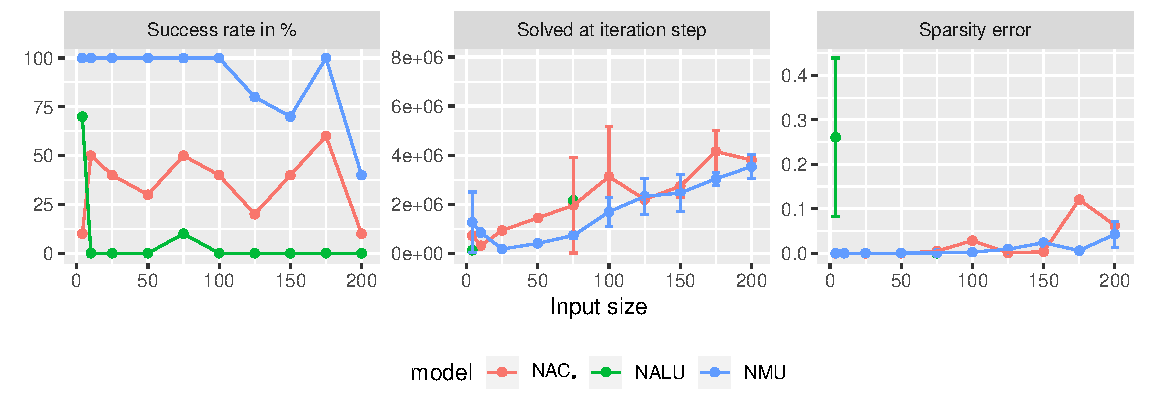
\includegraphics[width=\linewidth,trim={0 1.3cm 0 0},clip]{results/simple_function_static_input_size.pdf}
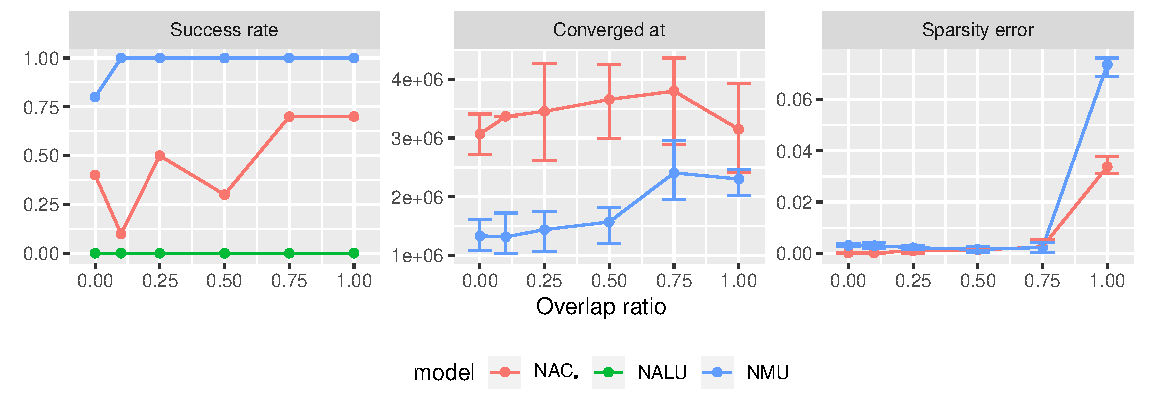
\includegraphics[width=\linewidth,trim={0 1.3cm 0 0.809cm},clip]{results/simple_function_static_overlap.pdf}
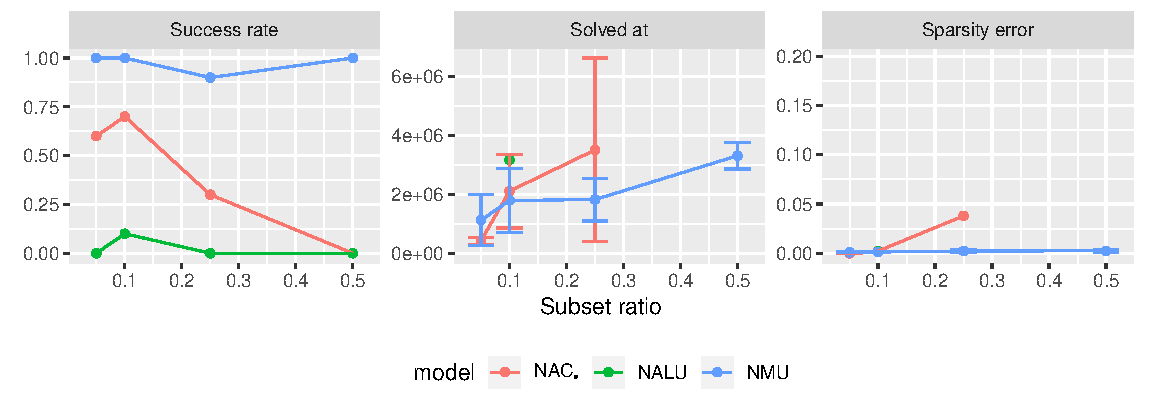
\includegraphics[width=\linewidth,trim={0 1.3cm 0 0.809cm},clip]{results/simple_function_static_subset.pdf}
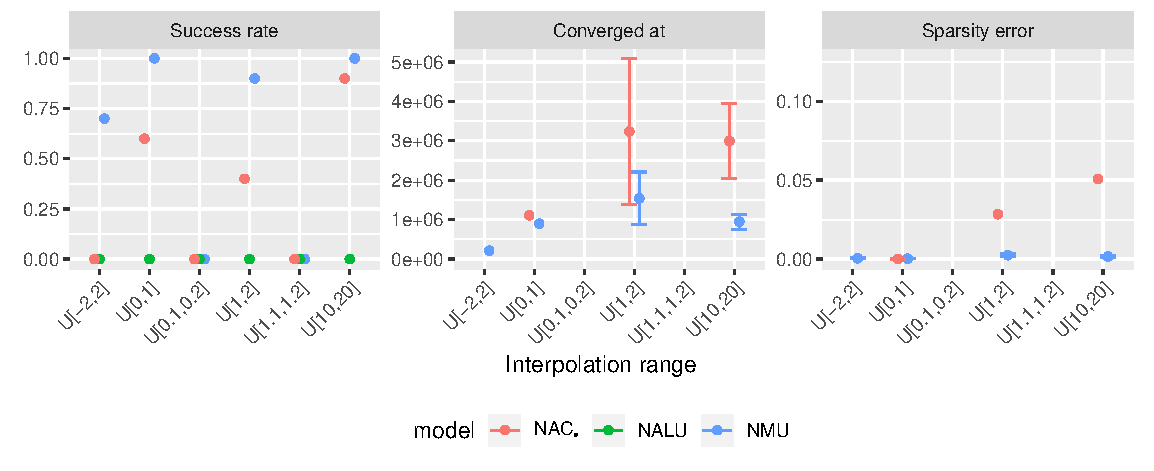
\includegraphics[width=\linewidth,trim={0 0 0 0.809cm},clip]{results/simple_function_static_range.pdf}
\caption{Shows the effect of the dataset parameters. For each interpolation range, the following extrapolation ranges are used: ${\mathrm{U}[-2,2] \rightarrow \mathrm{U}[-6,-2] \cup \mathrm{U}[2,6]}$, ${\mathrm{U}[0,1] \rightarrow \mathrm{U}[1,5]}$, ${\mathrm{U}[0.1,0.2] \rightarrow \mathrm{U}[0.2,2]}$, ${\mathrm{U}[1,2] \rightarrow \mathrm{U}[2,6]}$, ${\mathrm{U}[10, 20] \rightarrow \mathrm{U}[20, 40]}$.}
\label{fig:simple-function-static-boundary}
\end{figure}
